%%%%%%%%%%%%%%%%%%%%%%%%%%%%%%%%%%%%%%%%%%%%%%%%%%%%%%%%%%%%%%%%%%%%%%%%%%%%%%%%
%2345678901234567890123456789012345678901234567890123456789012345678901234567890
%        1         2         3         4         5         6         7         8
\documentclass[letterpaper, 10 pt, conference]{ieeeconf}  % Comment this line out
                                                          % if you need a4paper
%\documentclass[a4paper, 10pt, conference]{ieeeconf}      % Use this line for a4

\usepackage{float}
                                                          % paper
% uso paquete bookmark para tener bien los outlines.
\usepackage{bookmark}

% Configuro el idioma.
\usepackage[utf8]{inputenc} % Importante para mantener acentos.
\usepackage[spanish, activeacute]{babel} % Requiere: texlive-lang-spanish. Por primera vez hay que ejecutar: texconfig init> log

% Paquete para poder usar acentos en $$.
\usepackage{mathtools}
%\setmathfont{XITS math}

% Para los diagramas de flujo
\usepackage{tikz}
\usetikzlibrary{shapes.geometric, arrows}

% Elementos del diagrama
\tikzstyle{startstop} = [rectangle, rounded corners, 
minimum width=6em, 
minimum height=2em,
text centered, 
draw=black, 
fill=red!30]

\tikzstyle{io} = [trapezium, 
trapezium stretches=true, % A later addition
trapezium left angle=70, 
trapezium right angle=110, 
minimum width=6em, 
minimum height=2em, text centered, 
draw=black, fill=blue!30]

\tikzstyle{block} = [rectangle, 
minimum width=8em, 
minimum height=3em, 
text centered, 
text width=7.5em, 
draw=black, 
fill=white!30]

\tikzstyle{def} = [rectangle, 
minimum width=14em, 
minimum height=3em, 
text centered, 
text width=12em, 
draw=black, 
fill=purple!30]

\tikzstyle{swap_proccess} = [rectangle, 
minimum width=8em, 
minimum height=2em, 
text centered, 
text width=8em, 
draw=black, 
fill=orange!30]

\tikzstyle{process} = [rectangle, 
minimum width=6em, 
minimum height=2em, 
text centered, 
text width=6em, 
draw=black, 
fill=orange!30]

\tikzstyle{decision} = [diamond, 
minimum width=6em, 
minimum height=6em, 
text centered, 
draw=black, 
fill=green!30]
\tikzstyle{arrow} = [thick,->,>=stealth]

\usepackage{siunitx}

% package to get \url
\usepackage{hyperref}
\hypersetup{
  colorlinks=true,
  linkcolor=magenta,
  filecolor=magenta,
  citecolor=magenta,      
  urlcolor=magenta,
}

% Graficos electrónicos
\usepackage[RPvoltages]{circuitikz}

\IEEEoverridecommandlockouts                              % This command is only
                                                          % needed if you want to
                                                          % use the \thanks command
\overrideIEEEmargins
% See the \addtolength command later in the file to balance the column lengths
% on the last page of the document

\usepackage{graphicx}
\usepackage{graphics}

% styling for matlab/octave code.
\usepackage{matlab-prettifier}
% Configuracion, con esto puede agregar ñ.
\lstset{
  literate={ñ}{{\~n}}1
}

\usepackage{listings}

% The following packages can be found on http:\\www.ctan.org
%\usepackage{graphics} % for pdf, bitmapped graphics files
%\usepackage{epsfig} % for postscript graphics files
%\usepackage{mathptmx} % assumes new font selection scheme installed
%\usepackage{times} % assumes new font selection scheme installed
\usepackage{amsmath} % assumes amsmath package installed
%\usepackage{amssymb}  % assumes amsmath package installed

\title{\LARGE \bf Amplificador de audio con boostrapping}

\author{
  Tom\'as Vidal\\
  {\it Circuitos Electróicos II}\\
  {\it Facultad de Ingenier\'ia, UNLP, La Plata, Argentina.}\\
  {\it 30 de Septiembre, 2024.}
}                                            % <-this % stops a space

\begin{document}
\maketitle
\thispagestyle{empty}
\pagestyle{empty}

\section{Placa}
\begin{figure}[htpb]
  \centering
  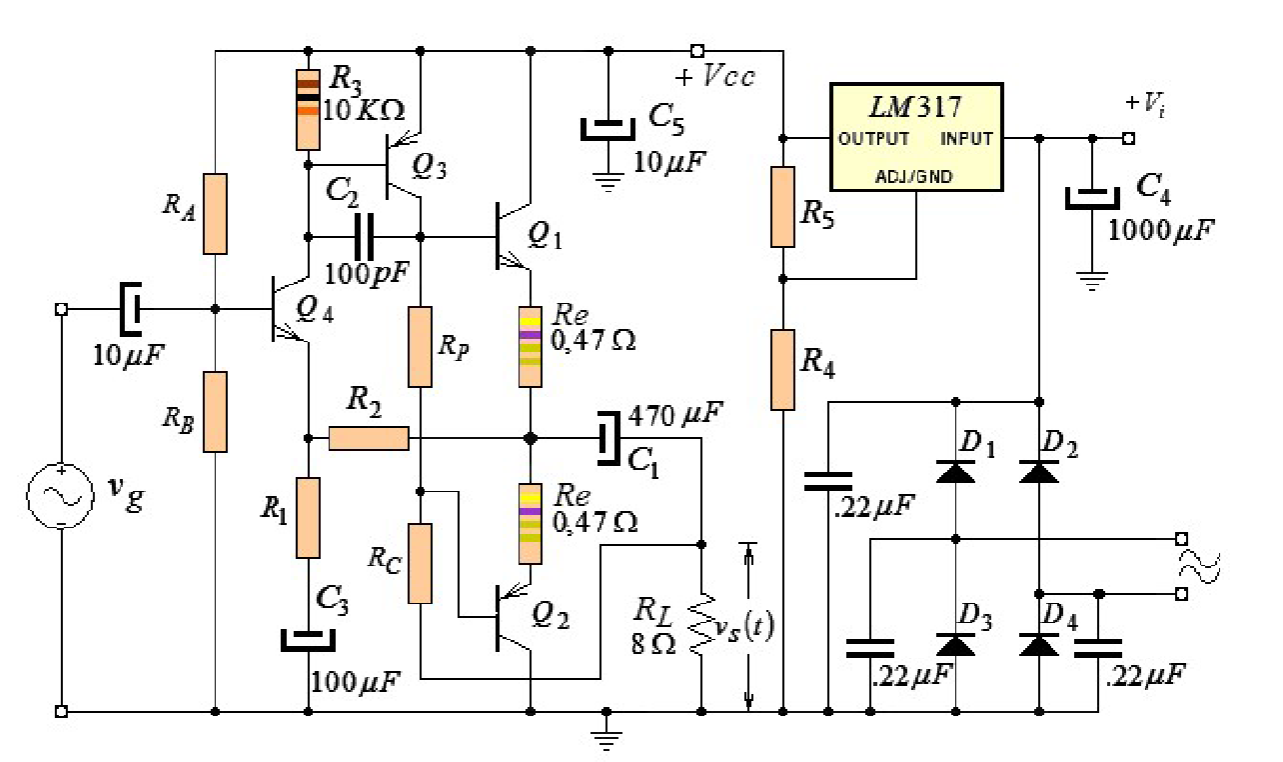
\includegraphics[width=0.43\textwidth]{./imagenes/placa.png}
  \caption{Esquemático del circuito a diseñar}
  \label{fig:placa}
\end{figure}
El circuito a implementar consiste de una \textbf{fuente de alimentación}, un \textbf{par complementario} que amplifica la corriente, y dos etapas de \textbf{emisor común} realimentadas que amplifican tensión. Además hay una rama de realimentación de \textbf{boostrapping}. La dos etapas de amplificación hacen que se tenga mucha ganacia de lazo directo, así la red beta dada por $R_1$, $R_2$ y $C_3$ puede establecer la ganancia de lazo cerrado.

\begin{figure}[htbp]
  \centering
  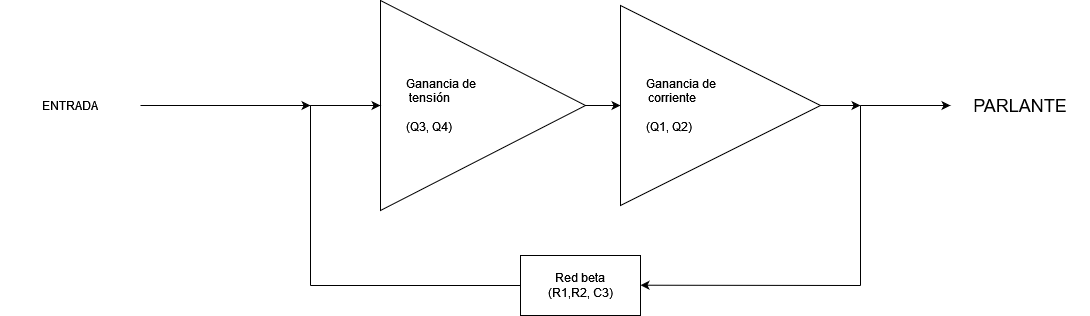
\includegraphics[width=0.43\textwidth]{./imagenes/diag_realimentacion.png}
  \caption{Diagrama en bloques del sistema}
\end{figure}


\section{Cálculo de los parámetros de diseño}
\subsection{Fuente de alimentación}
\begin{figure}[H]
  \centering
  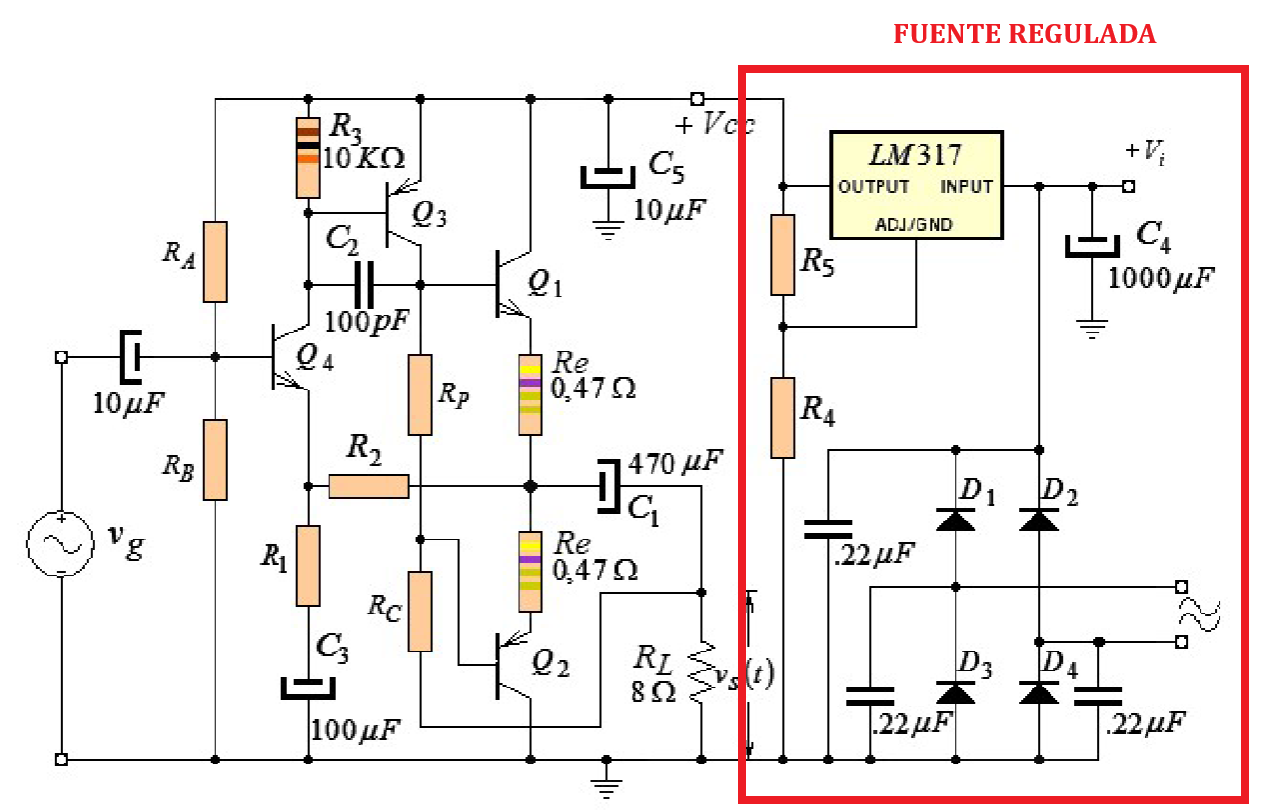
\includegraphics[width=0.43\textwidth]{./imagenes/placa_fuente.png}
  \caption{Sección de la fuente regulada}
  \label{fig:placa_fuente}
\end{figure}

Especificaciones de entrada:
\begin{itemize}
  \item{$220V_{ef} AC$ a $50Hz$ con un ripple del $10\%$}
\end{itemize}
Requerimientos de salida:
\begin{itemize}
  \item{13V con ripple máximo de $8\%$}
\end{itemize}

Para cumplir con estas condiciones se empleó un análisis con las siguientes consideraciones:
\begin{itemize}
  \item{60V y 1.5A máximos en el LM317}
  \item{3V mínimos entre entrada y salida del LM317}
  \item{La corriente de ajuste del LM317 tiene que ser del orden de los $\qty{}{\micro\ampere}$, contra la de $R_1$ y $R_2$ que debe ser del orden de los $mA$}
\end{itemize}

Partiendo de que en la salida del regulador se tiene una carga de \qty{50}{\ohm}, y se quiere una tensión \textit{estable} de \qty{13}{\volt}; se puede calcular la corriente máxima en la carga, para lo cual se consideró que la carga puede variar un $10\%$ (como medida de seguidad, ya que menor carga será mayor corriente), es decir, puede variar a \qty{45}{\ohm} en el peor caso, resultando así en una corriente máxima de aproximadamente \qty{300}{\milli\ampere}. \\
Sabiendo la tensión mínima del regulador, y agregandole un márgen de seguridad de \qty{1}{\volt}; se calcula la resistencia equivalente del LM317: 
\begin{equation} \label{eq:lm317_resistance}
  R_{LM317} = \frac{4V}{300mA} \cong \qty{15}{\ohm}
\end{equation}

Por lo que se puede calcular la tensión máxima requerida en el secundario con las curvas de \textbf{Schade}; haciendo la carga del rectificador filtrado \qty{65}{\ohm} (la carga original de \qty{50}{\ohm} en serie con los \qty{15}{\ohm}), como se muestra en la figura \ref{fig:lm317_como_resistencia}
\begin{figure}[H]
  \centering
  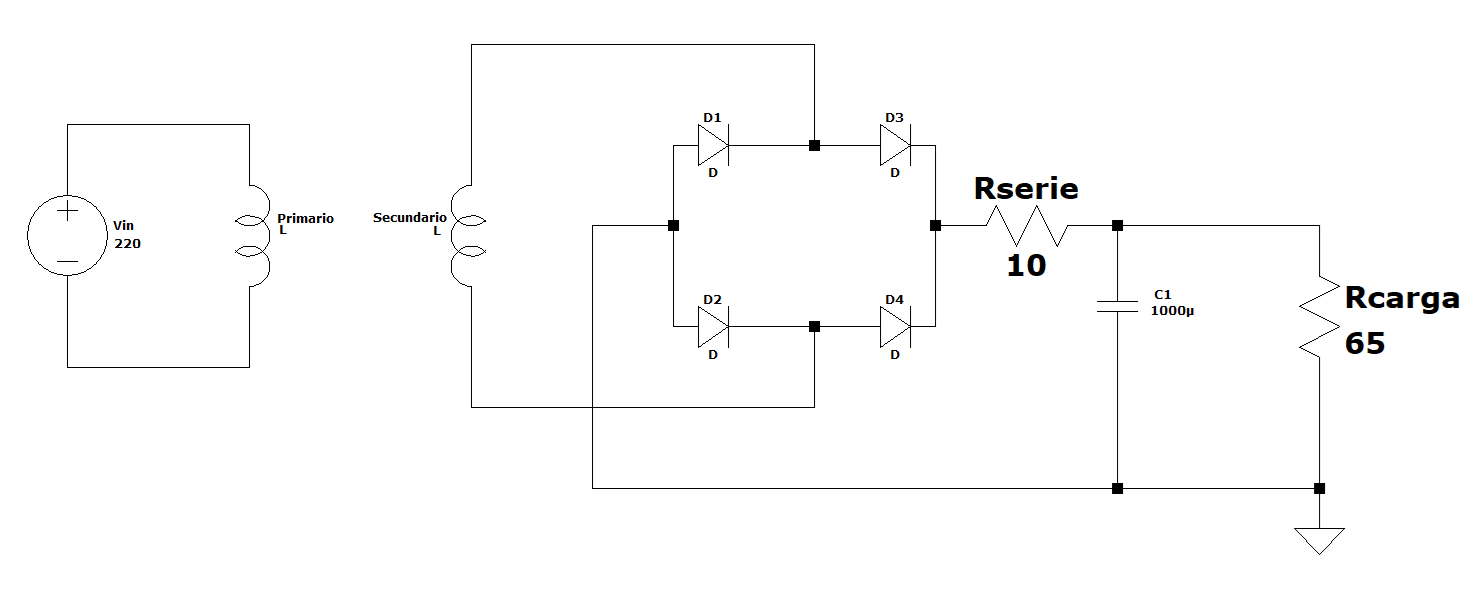
\includegraphics[width=0.43\textwidth]{./imagenes/circ_eq_lm137_carga.png}
  \caption{Circuito equivalente con LM317 como resistencia}
  \label{fig:lm317_como_resistencia}
\end{figure}

Tomando $\frac{R_s}{R_{carga}}\% = \frac{10}{65}*100 \cong 15\%$ ($R_s$ es un dato conocido); y calculando $wR_{carga}C \cong 20$, se puede obtener de las curvas de \textbf{Schade} el ripple en el capacitor, que será aproximadamente de $3\%$, y la tensión máxima del secundario, que será de $26V$ pico para el peor caso, es decir cuando en el primario se tenga $90\%$ de la tensión. Con estos datos se puede obtener la relación de espiras entre el primario y el secundario del transformador: \\
\textit{Se debe considerar que en el puente de diodos hay caida de tensión también (aproximadamente de 1.5V). Por eso resulta tan alta la tensión del secundario.}

\begin{equation}
  \frac{V_1}{V_2} = \frac{N_1}{N_2} = N \cong 10.78
\end{equation}

\begin{figure}[H]
  \centering
  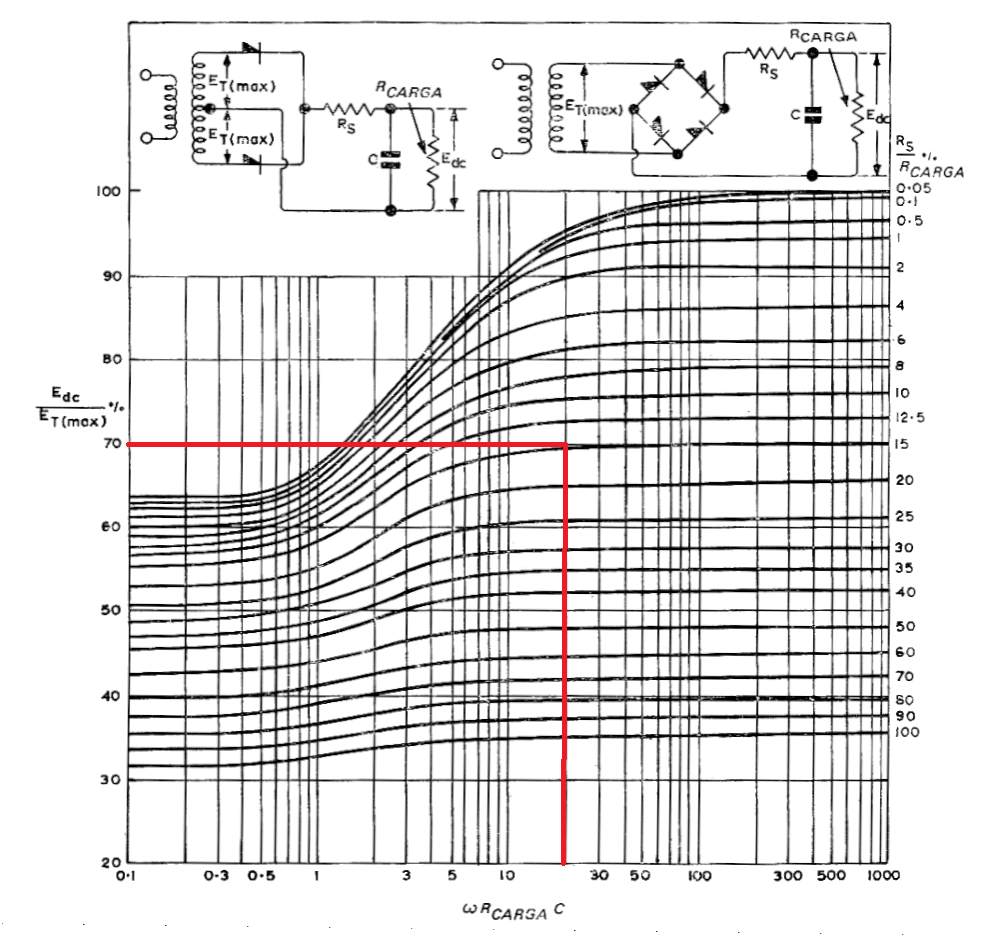
\includegraphics[width=0.43\textwidth]{./imagenes/schade_edc_et.png}
  \caption{Curva de Schade}
  \label{fig:schade_edc_sobre_etmax}
\end{figure}

\textit{Los cálculos anteriores se consideraron para el caso de carga nominal y carga mínima, que es el peor caso, cuando más corriente se demanda en la carga. $N \cong 10.78$ es el caso pesimista.} \\

\textit{Se observa que los cálculos de tensión dan resultado altos pero también se simularon, y para tensiones menores el regulador empieza a fallar (no suministra la tensión aproximada de 13V a la salida)}

\begin{figure}[H]
  \centering
  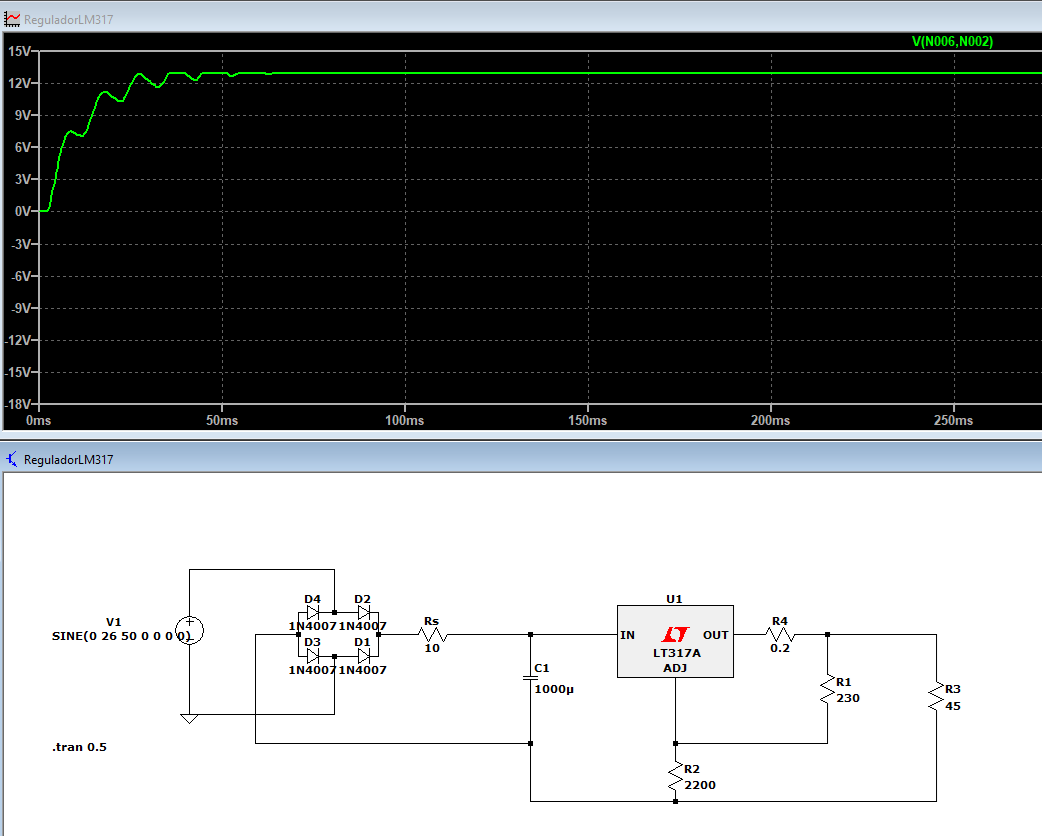
\includegraphics[width=0.43\textwidth]{./imagenes/sim_fuente_bien.png}
  \caption{Fuente alimentada con 26V pico de secundario}
\end{figure}

\begin{figure}[H]
  \centering
  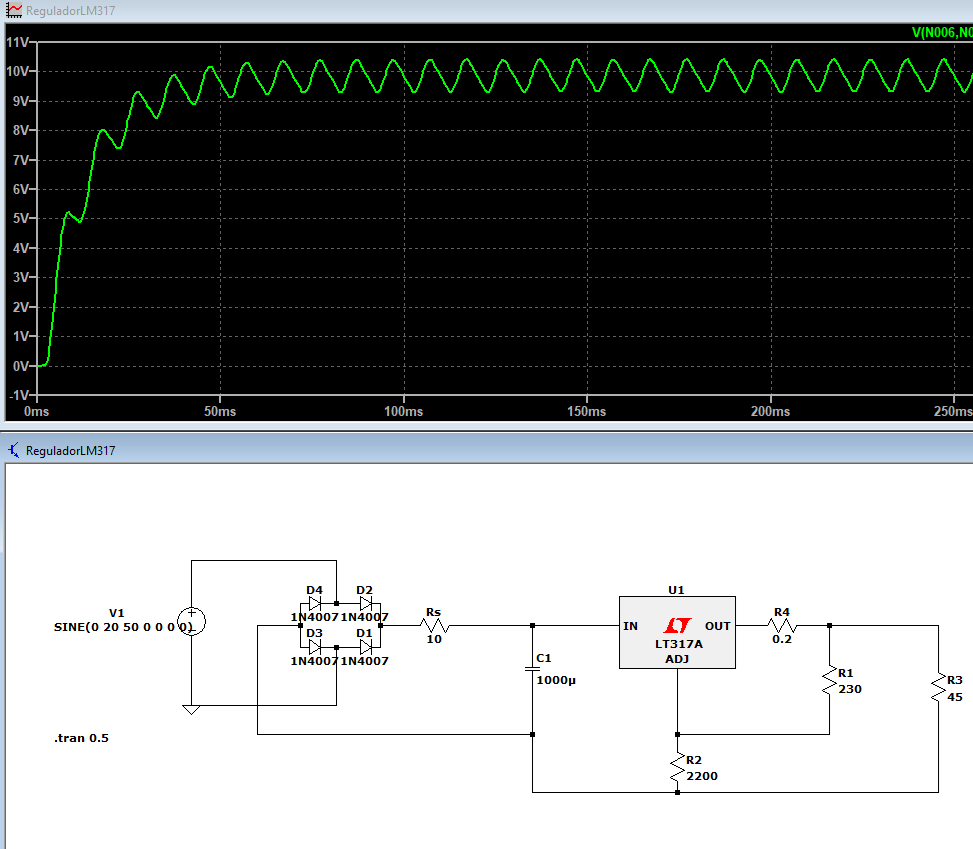
\includegraphics[width=0.43\textwidth]{./imagenes/sim_fuente_mal.png}
  \caption{Fuente alimentada con 20V pico de secundario}
\end{figure}

\begin{figure}[H]
  \centering
  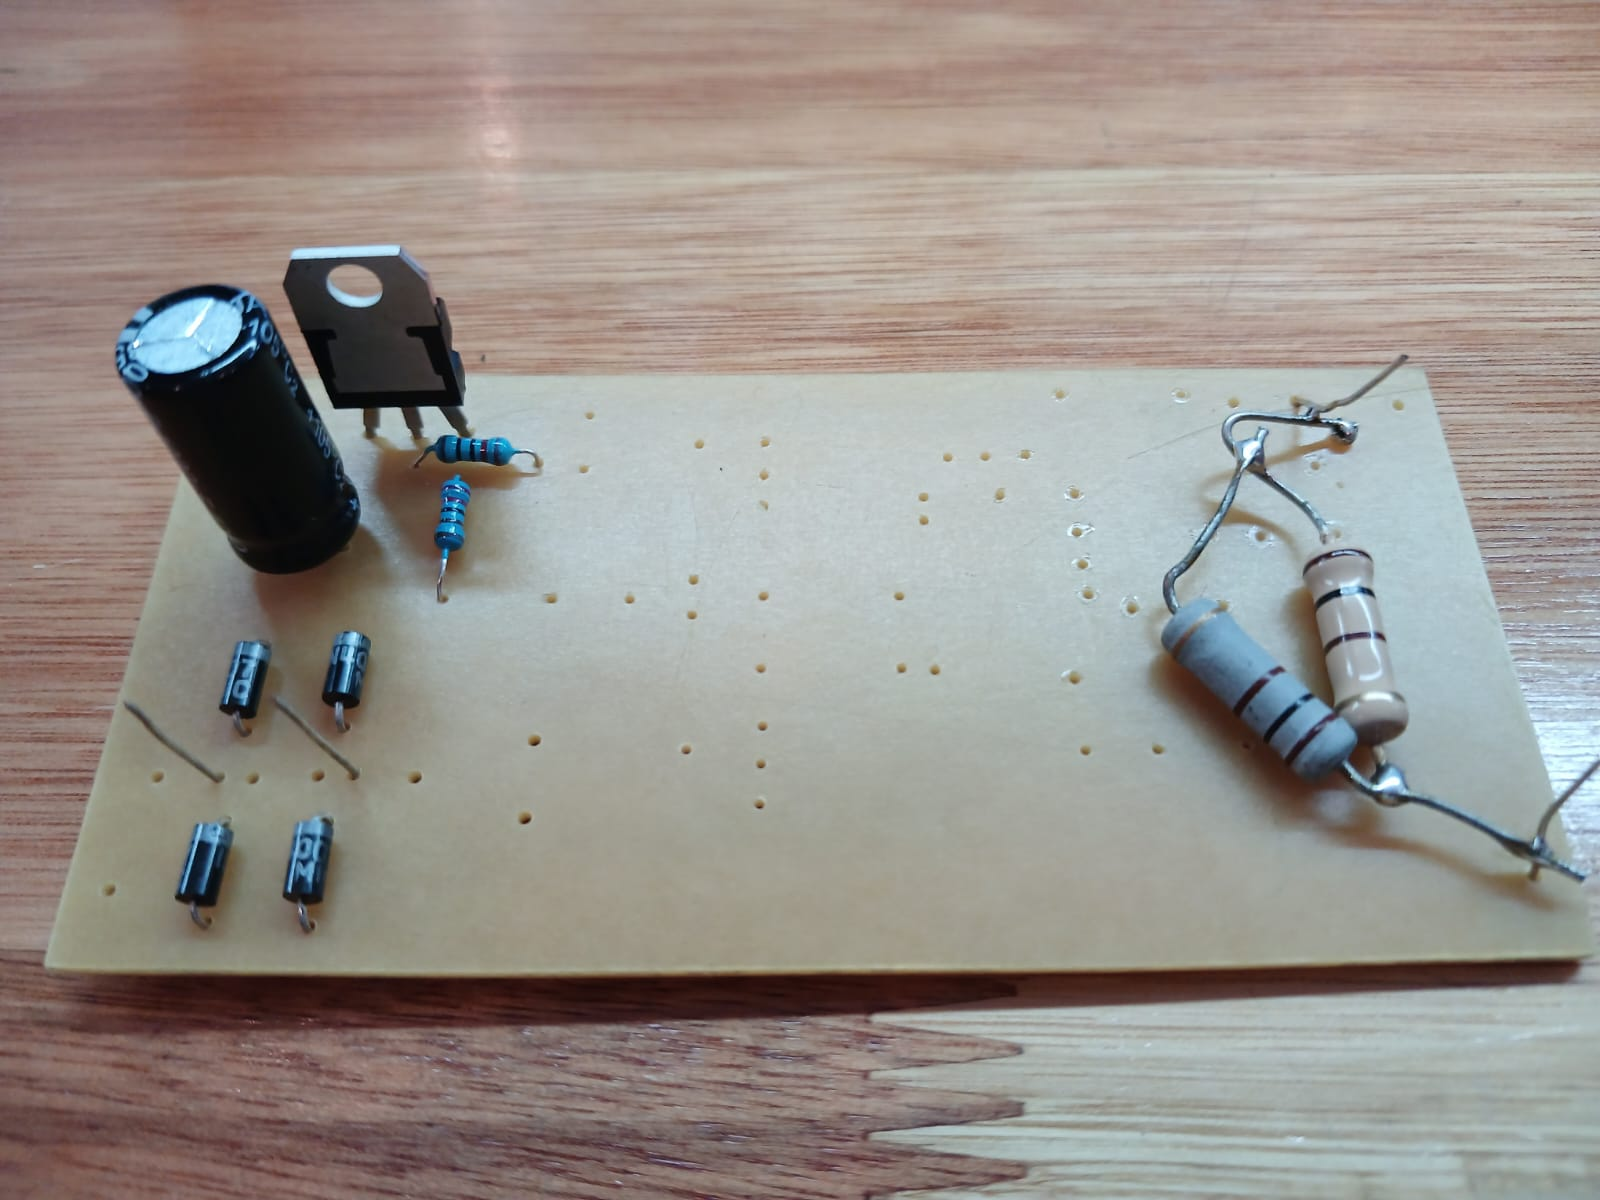
\includegraphics[width=0.43\textwidth]{./imagenes/fuente_cargada.jpeg}
  \caption{Fuente soldada y cargada con \qty{50}{\ohm}}
\end{figure}

\textit{Lamentablemente el regulador LM317 estaba roto, por lo que no se pudo hacer funcionar correctamente la fuente.}

\subsection{Amplificador de tensión realimentado}
\begin{figure}[H]
  \centering
  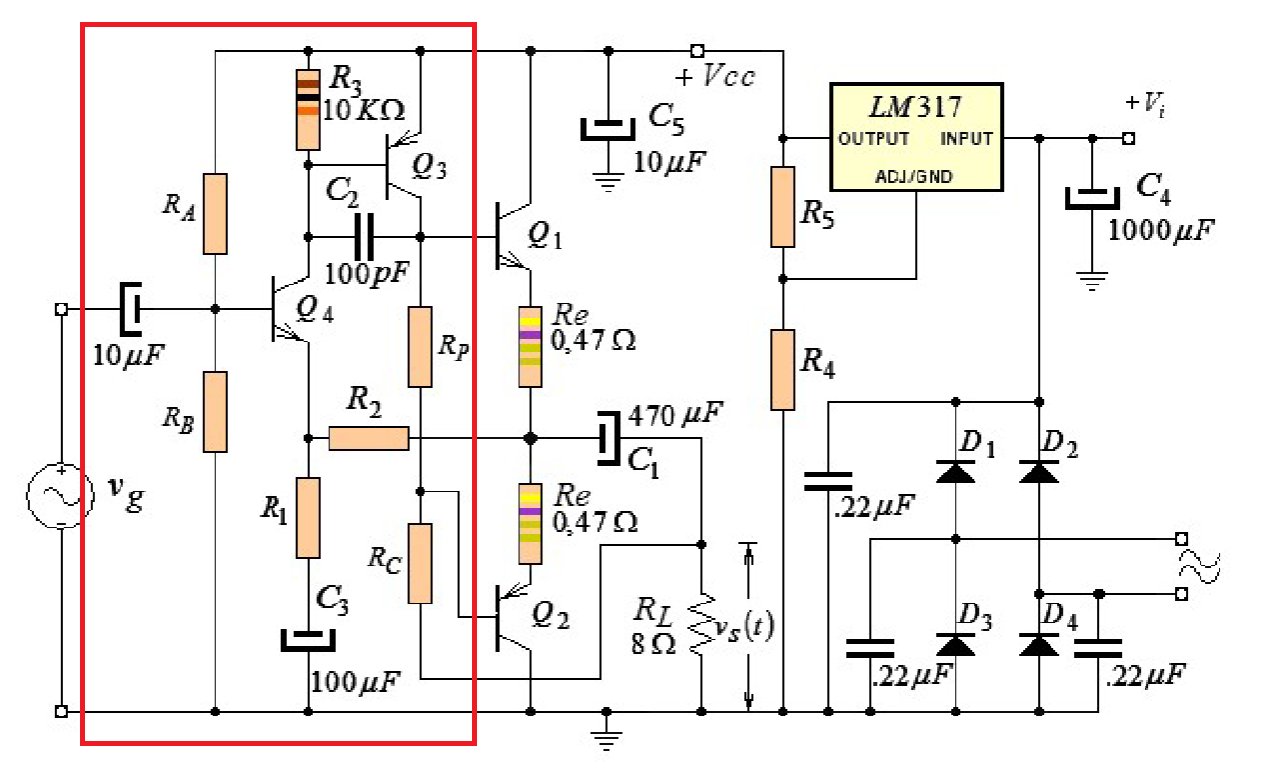
\includegraphics[width=0.43\textwidth]{./imagenes/placa_ampli_realimentado.png}
  \caption{Sección de amplificación de tensión realimentada}
  \label{fig:ampl_tension_reali}
\end{figure}
Los transistores $Q_3$ y $Q_4$, en configuración \textbf{emisor común}, en combinación con el divisior resistivo $R_1$ y $R_2$; forman un \textbf{amplificador de tensión realimentado negativamente}(\ref{fig:circ_eq_ampli_reali}). El propósito del mismo es tener una ganacia en tensión elevada, proporcionada por $Q_3$ y $Q_4$, y la realimentación estabiliza la tensión a coste de ganancia. Estos componentes se pueden pensar como el siguiente circuito equivalente (fig \ref{fig:circ_eq_ampli_reali}), tanto se cumpla que la gananacia de tensión proporsionada por $Q_3$ y $Q_4$ sea lo \textit{suficientemente}\footnote{Es decir que se cumpla $a\beta \gg 1$. Se puede asumir que lo hace, ya que las etapas de emisior común se ajustan para que así lo sea.} elevada.

\begin{figure}[H]
  \centering
  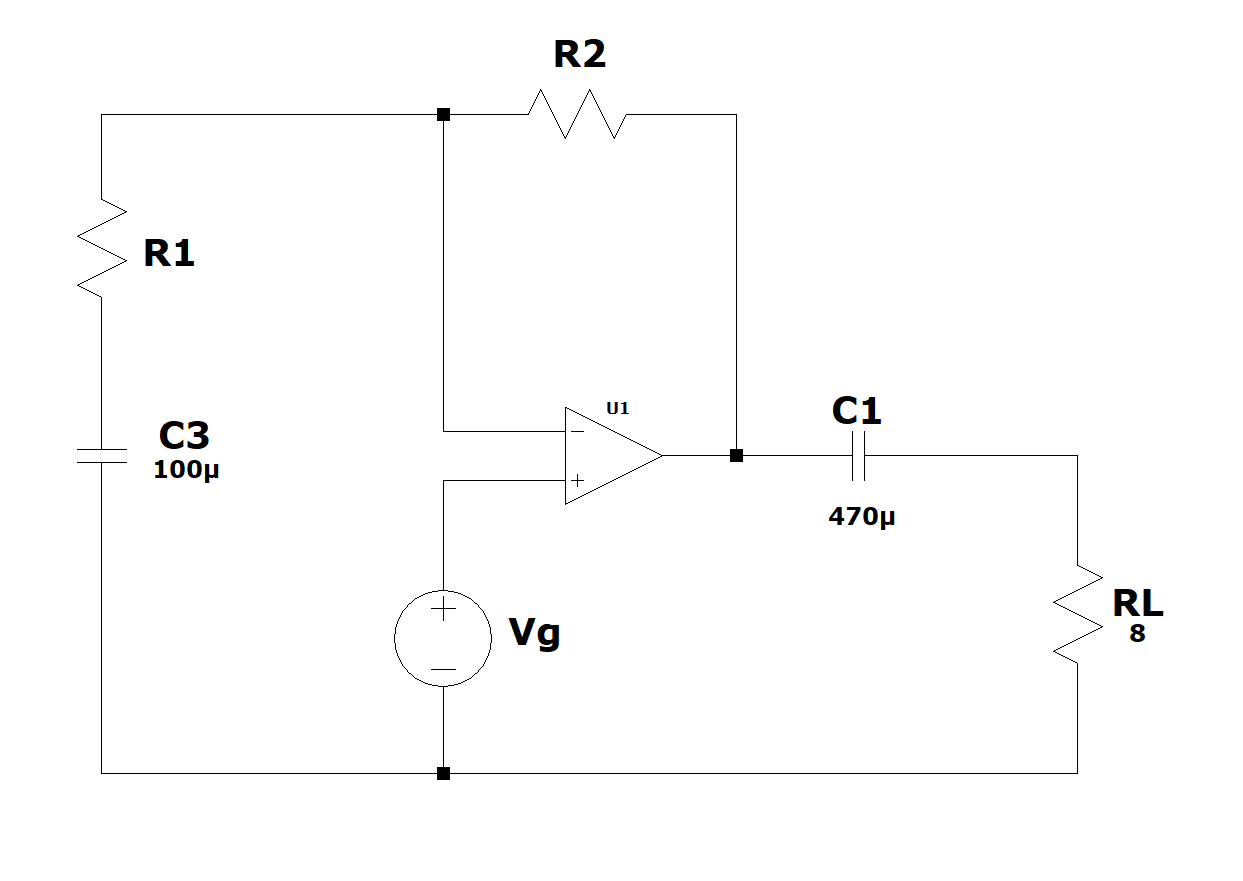
\includegraphics[width=0.43\textwidth]{./imagenes/circ_eq_ampli_real.png}
  \caption{Circuito equivalente del amplificador realimentado}
  \label{fig:circ_eq_ampli_reali}
\end{figure}

La ganacia de este circuito equivalente \textit{(en frecuencias medias)} se puede ajustar fácilmente con $R_1$ y $R_2$, sabiendo:
\begin{equation} \label{eq:ganancia_ampli_real}
  G_0 = 1 + \frac{R_2}{R_1}
\end{equation}

Además para ajustar $R_1$ se consideró que el polo de baja frecuencia que genera con $C_3$, debe ser de menor frecuencia que el que genera $R_L$ y $C_1$. Por lo que si se quiere que $f_1 = \frac{1}{2{\pi}R_LC_1} \cong 42Hz$ sea dominante (una década de separación en frecuencia), entonces $f_{2} = \frac{1}{2{\pi}R_1C_3} \cong 4Hz$, por lo tanto $R_1 \cong \qty{398}{\ohm}$. \\
Entonces empleando la ecuación \ref{eq:ganancia_ampli_real} se puede obtener $R_2 \cong \qty{6}{\kilo\ohm}$. \\

Para calcular $R_C$ se consideró el estado en el que $Q_3$ se encuentra \textit{prácticamente} en corte (es decir la corriente de colector es la menor posible), quedando el siguiente circuito equivalente (el capacitor $C_1$ se considera con tensión constante para este caso):

\begin{figure}[H]
  \centering
  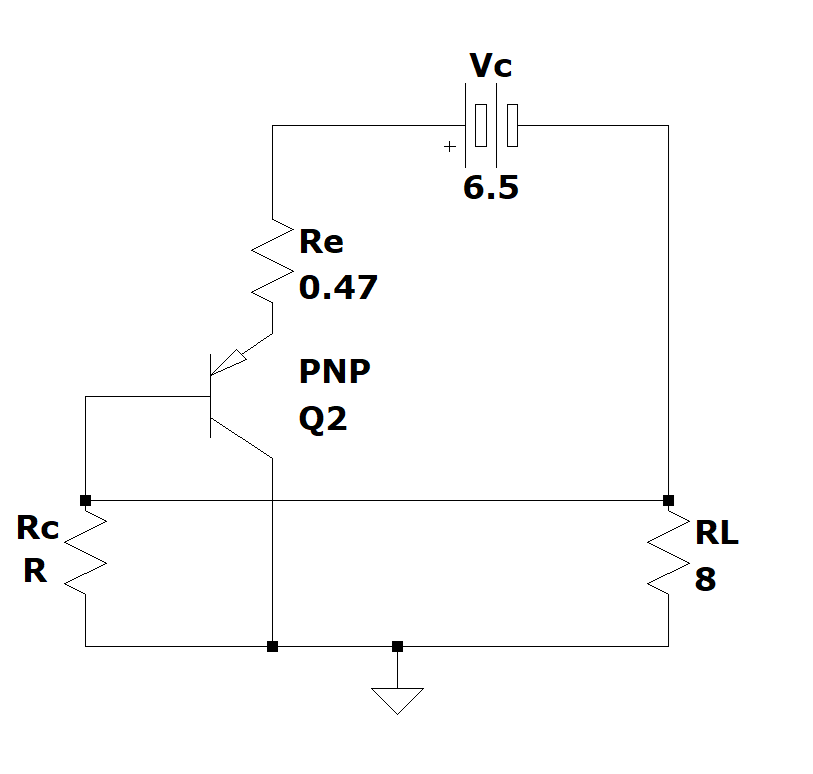
\includegraphics[width=0.43\textwidth]{./imagenes/circ_calculo_rc.png}
  \caption{Circuito equivalente del amplificador realimentado}
\end{figure}

Donde resolviendo la maya de $R_L$ y luego la de $R_C$ se puede obtener el valor de $R_C \cong \qty{1100}{\ohm}$. \\

Luego, considerando que la caída de tensión sobre $R_p$ debe ser de \qty{750}{\milli\volt}, y sabiendo que la corriente cuando no hay señal es de aproximadamente \qty{5}{\milli\ampere}, se obtuvo $R_p \cong \qty{140}{\ohm}$. \\

Para poder obtener los valores de $R_A$ y $R_B$, que polarizan al transistor $Q_4$ y establecen la tensión del capacitor cuando no hay señal (se desean que hayan 6V), se consideró que la corriente que debe pasar por $R_A$ y $R_B$ debe ser \textit{mucho} más grande que la corriente que entra por la base de $Q_4$, es decir se $I_{B4}$ de los \qty{}{\micro\ampere}, entonces con que la corriente por $R_A$ y $R_B$ se de los \qty{10}{\milli\ampere} se puede ignorar $I_{B4}$, por lo que la suma de estas resistencias debe de ser del orden de los \qty{}{\kilo\ohm}. Además se debe considerar que si no hay señal y se tiene la tensión deseada en el capacitor, por $R_2$ no hay corriente, entonces en el emisor de $Q_4$ la tensión debe ser la deseada de 6V, de esta manera se sabe que la tensión del divisor resistivo debe de ser $6V+V_{BE4}$, por lo que las resistencias son:
\begin{equation*}
  \begin{cases*}
    R_A + R_B = \frac{13V}{10mA} = \qty{1300}{\ohm} \\
    \frac{R_B 13V}{R_A+R_B} = 6.55V
  \end{cases*}
\end{equation*}

Resolviendo:

\begin{equation*}
  R_A \cong \qty{645}{\ohm}
\end{equation*}
\begin{equation*}
  R_B \cong \qty{655}{\ohm}
\end{equation*}

\subsection{Valores reales}
Todos los valores teóricos calculados previamente fueron reemplazados por valores comerciales reales, de la serie de resistores E12 (al $10\%$), a excepción de las resistencias $R_4$ y $R_5$ que fueron elegidas al $1\%$.

\begin{itemize}
  \item{$R_4$ = \qty{2200}{\ohm}}
  \item{$R_5$ = \qty{220}{\ohm}}
  \item{$R_A$ = \qty{680}{\ohm}}
  \item{$R_B$ = \qty{680}{\ohm}}
  \item{$R_2$ = \qty{6200}{\ohm}}
  \item{$R_1$ = \qty{470}{\ohm}}
  \item{$R_p$ = \qty{150}{\ohm}}
  \item{$R_c$ = \qty{1200}{\ohm}}
\end{itemize}

\section{Simulaciones}

Para corroborar que todo funciona correctamente se hizo una simulación completa del circuito en LTSpice. En esta simulación se fueron viendo que los parámetros de diseño sean acordes, como por ejemplo la tensión que cae entre los terminales de $R_p$, o la tensión entre las resistencias $R_A$ y $R_B$. Todos los parámetros fueron acordes, con variaciones, pero no tan significativas, del orden del $15\%$ en el peor caso, y para los parámetros que no son tan importantes. \\

\textit{En la simulación la entrada es una sinusoide de 1Khz y 300mV pico, y actúa después de 1ms (así se puede observar el estado sin señal de entrada)}

\begin{figure}[H]
  \centering
  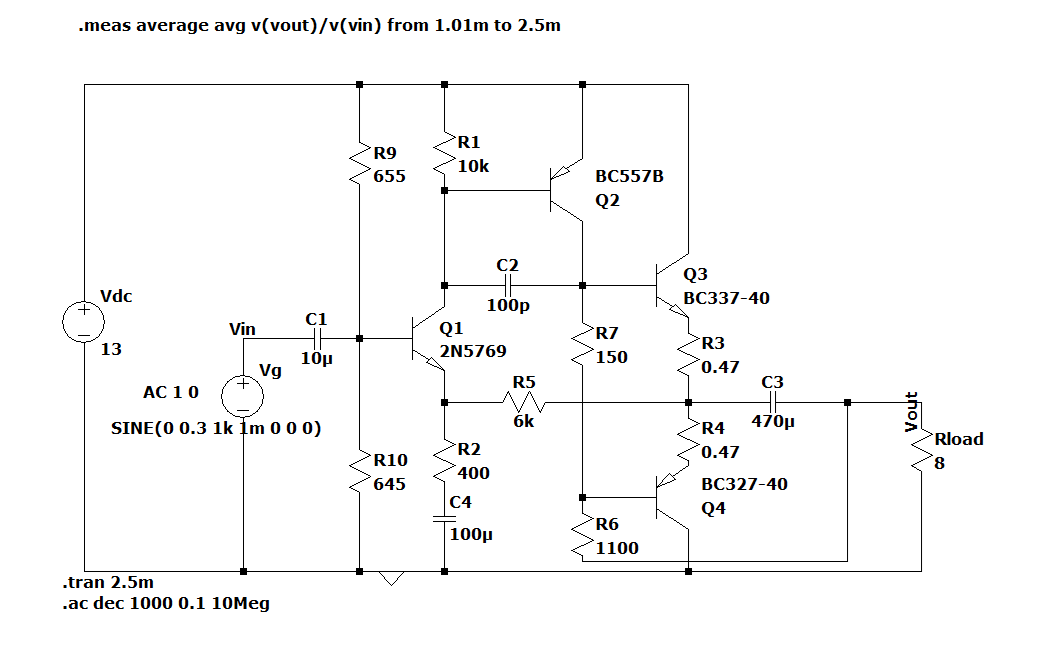
\includegraphics[width=0.43\textwidth]{./imagenes/placa_completa_simulacion.png}
  \caption{Simulación del circuito completo}
\end{figure}

\begin{figure}[H]
  \centering
  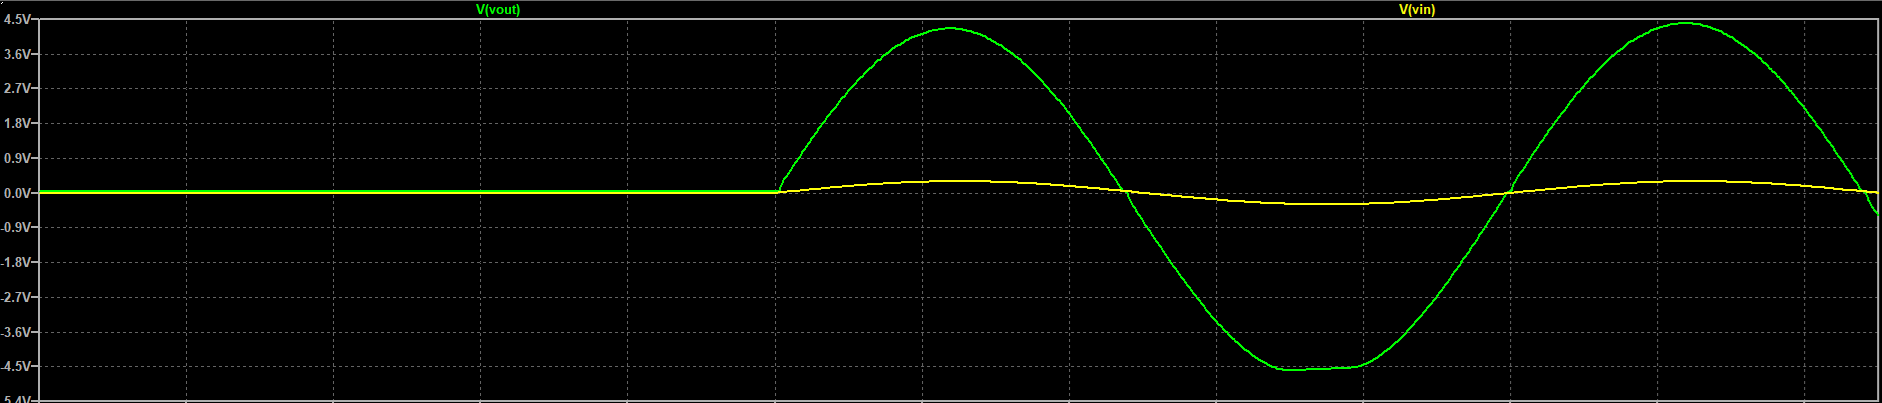
\includegraphics[width=0.43\textwidth]{./imagenes/sim_salida_entrada.png}
  \caption{Simulación señal de salida y entrada}
\end{figure}

\begin{figure}[H]
  \centering
  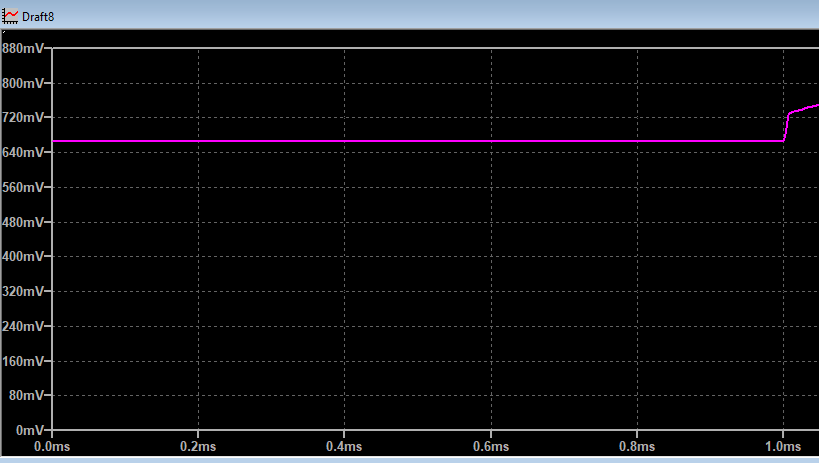
\includegraphics[width=0.43\textwidth]{./imagenes/sim_vp.png}
  \caption{Tensión de $V_P$ en la simulación}
\end{figure}

\begin{figure}[H]
  \centering
  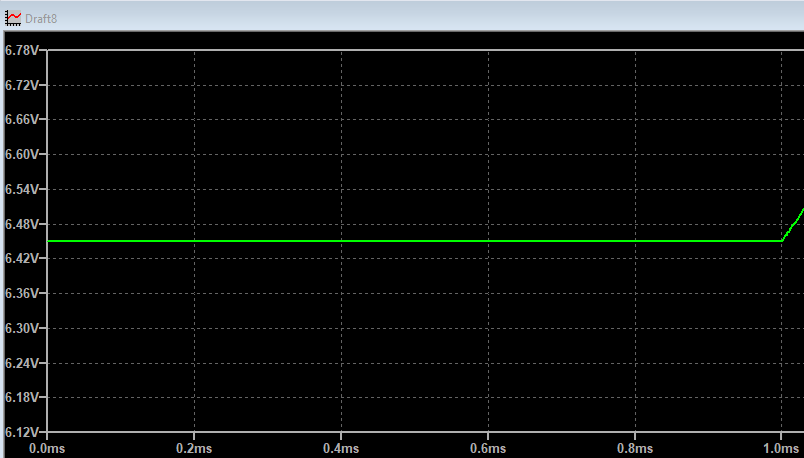
\includegraphics[width=0.43\textwidth]{./imagenes/sim_v_ra_rb.png}
  \caption{Tensión entre $R_A$ y $R_B$ en la simulación}
\end{figure}


\end{document}